
\documentclass{beamer}

\mode<presentation> {

% The Beamer class comes with a number of default slide themes
% which change the colors and layouts of slides. Below this is a list
% of all the themes, uncomment each in turn to see what they look like.

%\usetheme{default}
%\usetheme{AnnArbor}
%\usetheme{Antibes}
%\usetheme{Bergen}
%\usetheme{Berkeley}
%\usetheme{Berlin}
%\usetheme{Boadilla}
%\usetheme{CambridgeUS}
%\usetheme{Copenhagen}
%\usetheme{Darmstadt}
%\usetheme{Dresden}
%\usetheme{Frankfurt}
%\usetheme{Goettingen}
%\usetheme{Hannover}
%\usetheme{Ilmenau}
%\usetheme{JuanLesPins}
%\usetheme{Luebeck}
\usetheme{Madrid}
%\usetheme{Malmoe}
%\usetheme{Marburg}
%\usetheme{Montpellier}
%\usetheme{PaloAlto}
%\usetheme{Pittsburgh}
%\usetheme{Rochester}
%\usetheme{Singapore}
%\usetheme{Szeged}
%\usetheme{Warsaw}

% As well as themes, the Beamer class has a number of color themes
% for any slide theme. Uncomment each of these in turn to see how it
% changes the colors of your current slide theme.

%\usecolortheme{albatross}
%\usecolortheme{beaver}
%\usecolortheme{beetle}
%\usecolortheme{crane}
%\usecolortheme{dolphin}
%\usecolortheme{dove}
%\usecolortheme{fly}
%\usecolortheme{lily}
%\usecolortheme{orchid}
%\usecolortheme{rose}
%\usecolortheme{seagull}
%\usecolortheme{seahorse}
%\usecolortheme{whale}
%\usecolortheme{wolverine}

%\setbeamertemplate{footline} % To remove the footer line in all slides uncomment this line
%\setbeamertemplate{footline}[page number] % To replace the footer line in all slides with a simple slide count uncomment this line

%\setbeamertemplate{navigation symbols}{} % To remove the navigation symbols from the bottom of all slides uncomment this line
}

\usepackage{graphicx} % Allows including images
\usepackage{booktabs} % Allows the use of \toprule, \midrule and \bottomrule in tables
\usepackage{amsmath}
\usepackage{listings}
\usepackage{amssymb}
\setbeamertemplate{caption}[numbered]
%----------------------------------------------------------------------------------------
%	TITLE PAGE
%----------------------------------------------------------------------------------------

\title[Data and Design]{Research Design, Data, and Intro to R} % The short title appears at the bottom of every slide, the full title is only on the title page

\author[Barham]{Elena Barham} % Your name
\institute[Columbia]
{Columbia University} 
\date{\today} 

\begin{document}

\begin{frame}
\titlepage % Print the title page as the first slide
\end{frame}

%----------------------------------------------------------------------------------------
%	PRESENTATION SLIDES
%----------------------------------------------------------------------------------------

%------------------------------------------------

\begin{frame}
\frametitle{Roadmap}
\tableofcontents 
\end{frame} 
\section{Data Gathering}
\begin{frame}{Starting from a hypothesis}
To start research design:  
\begin{itemize} 
    \item Dependent variable(s)
    \item Independent variable(s) - variables of theoretical interest 
    \item Units of analysis 
\end{itemize}
\vspace{.5cm}
Some other questions to ask yourself:
\begin{itemize}
    \item What is my mechanism?
    \item What are the competing explanations? 
\end{itemize}
\end{frame} 

\begin{frame}{Making decisions as a researcher}
What we are looking for:
\begin{itemize}
    \item Clear mapping between theory and research design.   
    \item Strong identification strategy (if we aim to make causal claims).   
    \item Justified and well conceptualized measurements. 
    \item Attuned to the strengths and weaknesses of our designs. 
    \item Doable! 
\end{itemize}
\end{frame}



\begin{frame}{Operationalizing Variables}
Often our hypotheses involve relatively abstract concepts. For example, we might ask: "What is the effect of \textit{natural resource wealth} on \textit{corruption}? 
\begin{itemize}
    \item Conceptualization: defining the core concepts, i.e. What do we mean by corruption? 
    \item Operationalization: developing a research procedure to select and classify \textit{empirical representations} of a concept. 
    \item Measurement: implementing our operationalization strategy. 
\end{itemize}
\end{frame} 


\subsection{Measurement}
\begin{frame}{Good Measures}
\begin{itemize}
\item \textbf{Validity:} Does this measure what it claims to measure?
\item \textbf{Reliability:} Is this measure consistent? 
\begin{itemize}
    \item If I measure the same thing multiple times, does the measure yield the same results?
    \item Concerns about \textit{objectivity} of measures can often fall under this category of measurement issues.  
\end{itemize} 
\end{itemize}
\end{frame}

\begin{frame}{Good Measures}
\begin{itemize}
\item \textbf{Usability and interpretability:} Is this measure intelligible to my targeted reader? Are results from this measure clear to interpretations? 
\begin{itemize}
    \item Units?
    \item Subject to multiple interpretations (ratios?) 
\end{itemize}
\item \textbf{Economy:} Is this measurement strategy achievable given my other constraints?
\end{itemize} 
\end{frame}

\begin{frame}{Good Measures - Exercise}
Claim: ``Oil and other valuable natural resources make states more \textit{corrupt}". How do we measure corruption? 
\begin{itemize} 
\item \textbf{Measurement option 1:} Survey data of individuals living under the governments in question on their perceptions of institutional quality and experiences of corruption (i.e. AfroBarometer, AmericasBarometer). 
\item \textbf{Measurement option 2:} External expert coding on their perceptions of institutional quality (i.e. TI's Corruption Perceptions Index).
\item \textbf{Measurement option 3:} Measures of anti-corruption initiatives joined and legislation passed (i.e. membership in the Extractive Industries Transparency Initiative). 
\end{itemize} 
\end{frame}
\subsection{Sensitive items} 
\begin{frame}{Measuring Sensitive Concepts}
\begin{itemize}
    \item List experiments 
    \item Less sensitive downstream effects
    \item Expert opinions 
    \item Interviews \& trust of respondents 
\end{itemize}
\end{frame}

\begin{frame}{No great options}
\textbf{Discussion:} What are some strategies when we are not satisfied with existing measures but we are not able to collect original data? 
\end{frame} 

\begin{frame}{No great options}
\textbf{Discussion:} What are some strategies when we are not satisfied with existing measures? 
\begin{itemize}
    \item Validate across multiple measures
    \item Create indices of prior measures
    \item Contextualize our findings given weaknesses of measures 
\end{itemize}
\end{frame} 


\begin{frame}{Last Word on Measures}
 Measures don't need to be perfect, but we need to understand the \textbf{trade-offs} and \textbf{limitations} involved in our measurement strategies.
 \begin{itemize}
     \item Sometimes data driven.
     \item Sometimes an improvement in measurement is possible without sacrificing other aspects of the project. 
     \item Sometimes, the measure is the goal. 
 \end{itemize}
\end{frame}


\begin{frame}{Common Data Sources}
\textbf{Exercise:} In-class brainstorm! 
\end{frame}

\begin{frame}{Collecting Data}
Some approaches to collecting data:  
\begin{itemize}
    \item Novel survey
    \item Web scraping 
    \item Quantifying historical or qualitative data 
    \item Aggregating data from disparate sources 
    \item Requesting official data that hasn't been used for research but you suspect exists
    \item Other? 
\end{itemize}
\end{frame} 

\begin{frame}{Example - Data Collection}
\textbf{Research Question:} Do distributive political concerns help explain patterns of territorial conservation in Latin America? 
\begin{itemize}
    \item \textit{Measure}: We chose \textbf{protected areas} as our unit of analysis, which were the strictest level of conservation and relatively comparable across countries.  
\end{itemize}
\end{frame} 


\begin{frame}{Example - Data Collection}
\textbf{Research Question:} Do distributive political concerns help explain patterns of territorial conservation in Latin America? 
\begin{itemize} 
    \item \textit{Pre-existing data}: We found that the World Database on Protected Areas (WDPA) has a comprehensive list of global protected areas. Great! However, they did not have very much information about these territories...Alas! 
 \end{itemize}
\end{frame} 
\begin{frame}{Example - Data Collection}
\textbf{Research Question:} Do distributive political concerns help explain patterns of territorial conservation in Latin America? 
\begin{itemize} 
    \item \textit{New data}: We compiled comprehensive data on who owns and administers each protected area. 
    \begin{itemize}
        \item We wrote to individual environmental ministries to get their data. 
        \item We reached out to sub-national associations where environmental ministries failed.
        \item For the residual protected areas, we tracked down their creation laws and individually coded based on these documents. 
    \end{itemize}
\end{itemize}
\end{frame} 

\subsection{Data Structure}
\begin{frame}{Panel Design}
\begin{center} 
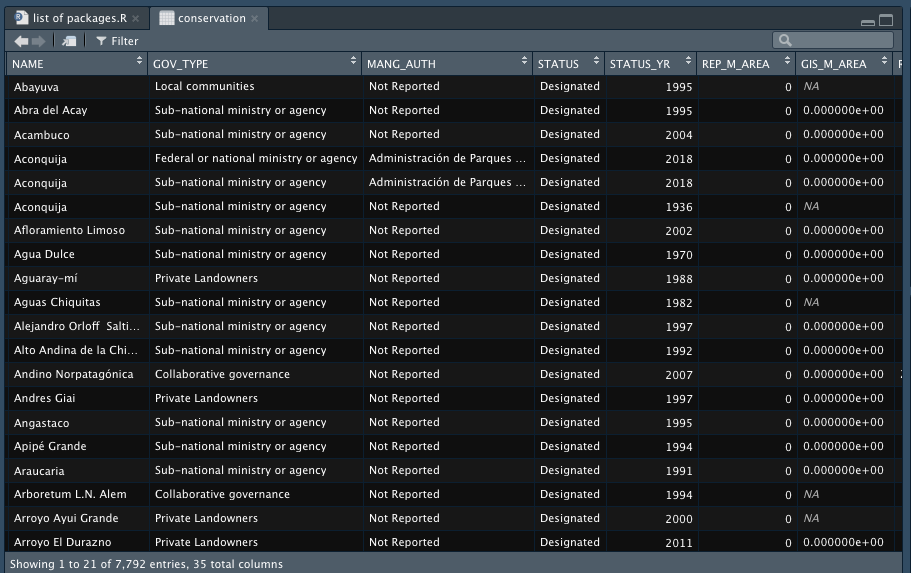
\includegraphics[width = .85\framewidth]{panel.png}
\end{center}
\end{frame}   
\begin{frame}{Missing Data}
\begin{itemize}
    \item Triage across sources. 
    \item Interpolation - strategies vary. 
    \item Work with complete data and theorize effect for results, external validity. What do we lose by dropping missing observations? Does this induce bias, or alter our confidence in our estimates? 
    \item Zoom out to a higher level of aggregation.  
\end{itemize}
\end{frame} 
\begin{frame}{Exercise}
\textbf{Try to write out the variable headings of a data set that could help you answer your question or test your hypothesis.}
\begin{itemize}
    \item What are your units of analysis?
    \item What information do you need about each unit?
    \item What is the scope of the data set (time periods, which units are in it?) 
\end{itemize}
\end{frame} 

\section{Data Analysis} 
\subsection{Coding Basics} 
\begin{frame}{Intro to R - Packages}
What are packages?
\begin{itemize}
    \item Loadable software within R or RStudio 
    \item Increase and broaden functionality of R
    \item Make it easier to do things that you could do in base R -- package mans someone else has gone to the trouble of writing the command for you!
\end{itemize}
How to know what package you need?
\begin{itemize}
    \item Usually we just look it up :) 
    \item Generally a process of trial and error 
\end{itemize}
\end{frame} 
\begin{frame}{Tidyverse}
Tidyverse is a suite of R packages that can make your life a lot easier. Functionality includes:
\begin{itemize}
    \item ggplot2 - functionality to make neat graphics 
    \item dplyr - data manipulation for common challenges 
    \item stringr - intuitive tools to work with strings (i.e. text variables) 
\end{itemize}
And more!
\end{frame} 
\begin{frame}{Loading Data}
Some possible formats:
\begin{itemize}
    \item .csv 
    \item .xlsx
    \item .Rda 
    \item .dta 
    \item shapefiles 
\end{itemize}
R can import many file types although some require packages to load. 
\end{frame}  
\subsection{Visualization and Data Exploration} 
\begin{frame}{Data Visualization}
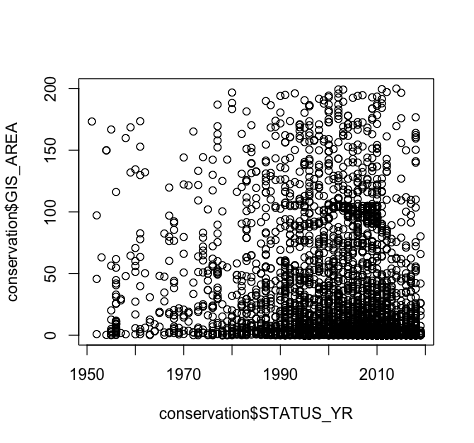
\includegraphics[width = .8\textwidth]{scatter_plot.png}
\end{frame} 
\begin{frame}{Data Visualization}
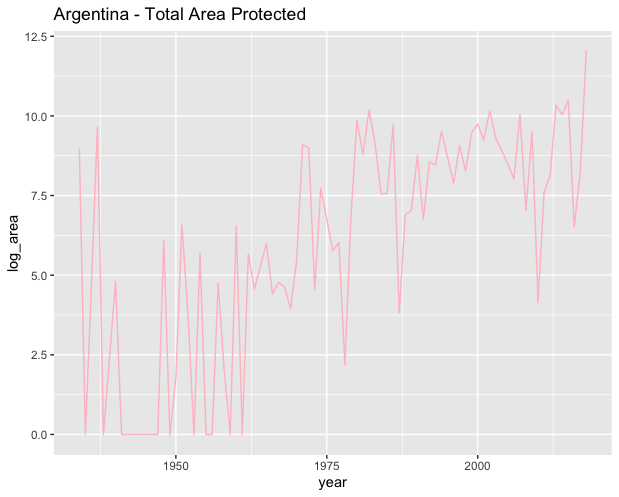
\includegraphics[width = .8\textwidth]{arg_tot.png}
\end{frame} 
\begin{frame}{Spatial Visualization}
\begin{columns}
\begin{column}{0.5\textwidth}
Why visualize spatially? 
\begin{itemize}
    \item Are there spatial patterns to the data?
    \item Are units independent (r.e. potential outcomes framework)? 
    \item Are there potential spillovers? 
\end{itemize}
\end{column}
\begin{column}{0.5\textwidth}
\begin{figure} 
\caption{Gang Density Per Block in Chicago (2015)}
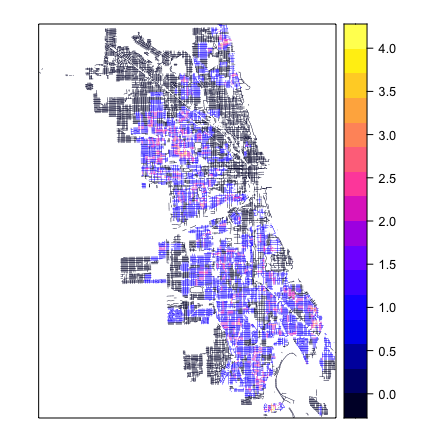
\includegraphics[width = .9 \textwidth]{gang_density.png}
\end{figure} 
\end{column}
\end{columns} 

\end{frame}
\subsection{Regression} 
\begin{frame}[fragile]{Regression Basics}
\begin{columns}
\begin{column}{0.5\textwidth}
$y_{i} = \beta_1 x_1 + \beta_2 x_2 + \epsilon_{i}$ \\ \vspace{.5cm} 
In R: \begin{itemize}
    \item lm(y $\thicksim$ $x_1$ + $x_2$, data = data) 
\end{itemize}
 \end{column}
 \begin{column}{0.5\textwidth}
Other packages for regression: 
\begin{itemize}
    \item glm - generalized linear models 
    \item experiment - experimental design and analysis 
    \item ivmodel, ivtools - for instrumental variable analysis 
\end{itemize}
\end{column}
\end{columns} 
\end{frame} 
\begin{frame}{Fixed Effects Models}
\textbf{Fixed effects:} Accounts for \textit{time-invariant} traits of units not captured by controls 
\begin{itemize}
    \item Compares variation within unit of FEs 
    \item Can help with omitted variable bias
    \item Level of FEs is a \textit{theoretical decision} 
    \item Multiple FEs may be justified
\end{itemize}
\end{frame} 
\begin{frame}{Interaction Terms}
\textit{Interaction terms:} These are useful when you think the effect of one variable depends on the value of another variable 
\begin{itemize}
    \item Differences-in-differences frameworks 
    \item Heterogeneous treatment effects 
    \item Different to mediation analysis 
\end{itemize}
\end{frame} 
\section{Reporting} 
\subsection{Graphs} 
\begin{frame}{Displaying Results}
\begin{center}
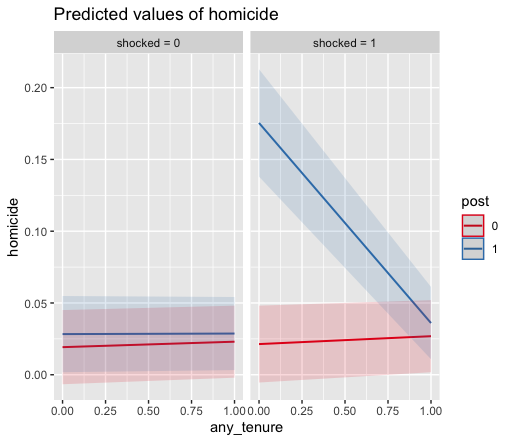
\includegraphics[width=.6\textwidth]{interaction_anytenure.png} 
\end{center} 
\end{frame} 
\subsection{Tables}
\begin{frame}{Regression Tables}
Stargazer can help make readable and nice tables in \LaTeX! 
\begin{table}[!htbp] \centering 
  \caption{Shocks increase violence in peripheral turf} 
  \label{} 
  \resizebox{.4\linewidth}{!}{
\begin{tabular}{@{\extracolsep{5pt}}lc} 
\\[-1.8ex]\hline 
\hline \\[-1.8ex] 
 & \multicolumn{1}{c}{\textit{Dependent variable:}} \\ 
\cline{2-2} 
\\[-1.8ex] & homicide \\ 
\hline \\[-1.8ex] 
shocked*post & 0.006$^{**}$ \\ 
  & (0.002) \\ 
  & \\  
 tot\_gangs & 0.002$^{*}$ \\ 
  & (0.001) \\ 
  & \\  
 shocked & 0.003$^{**}$ \\ 
  & (0.002) \\ 
  & \\ 
 post & 0.004$^{**}$ \\ 
  & (0.002) \\ 
  & \\ 
 Constant & 0.010 \\ 
  & (0.014) \\ 
  & \\ 
\hline \\[-1.8ex] 
Observations & 69,492 \\
Regional \& Seasonal FEs & Yes \\ 
Block controls & Yes \\ 
R$^{2}$ & 0.004 \\ 
Adjusted R$^{2}$ & 0.003 \\ 
\hline 
\hline \\[-1.8ex] 
\textit{Note:}  & \multicolumn{1}{r}{$^{*}$p$<$0.1; $^{**}$p$<$0.05; $^{***}$p$<$0.01} \\ 
\end{tabular} 
} 
\end{table} 
\end{frame} 

\section{Questions and Recap} 
\begin{frame}{Questions?}
Questions? 
\end{frame} 

\begin{frame}{Research and Epistemology}
\begin{itemize}
    \item Positivism  
    \begin{itemize}
        \item Core belief that concepts (like democracy) exist independently of inquiry and that social scientists' job is to measure and study these concepts to understand patterns within and across cases. Objective causes and effects exist. 
        \item Experimental and quasi-experimental methods,  focused on identifying causal effects 
        \item Descriptive, focused on identifying trends, associations, and relationships among theoretical variables of interest 
        \item Goal of absolute knowledge that accumulates to demonstrate objective truths  
    \end{itemize} 
    \end{itemize}
\end{frame}
\begin{frame}{Research and Epistemology}
\begin{itemize}
    \item Interpretivism  
    \begin{itemize}
        \item Core belief that concepts (like democracy) are socially embedded in the context of social scientists who study it, and whose goal is to clarify the way these concepts are used, meant, and produced in their historical and political contexts.  
        \item Descriptive, focused on conceptualization of specific, unique, and relative meanings 
        \item Goal of generating knowledge (relative to context, time, culture, etc) to describe subjective truths  
    \end{itemize}
\end{itemize}
\end{frame} 

\begin{frame}{Research Approaches for Positivists}
What do we mean by causal identification? 
\begin{itemize}
    \item Potentially ``causally identified": 
    \begin{itemize}
        \item Randomized controlled trials (RCTs)
        \item Quasi-experimental designs (differences-in-differences, regression discontinuity, matched comparisons/synthetic controls, instrumental variables analysis) 
    \end{itemize}
    \item Non-identified but still positivist:
    \begin{itemize}
        \item Correlation and regression 
        \item Qualitative methods with causal claims (ethnography, interview-based methods, case studies) 
    \end{itemize}
\end{itemize}
    
\end{frame}

\begin{frame}{Research Approaches for Interpretivists}
\begin{itemize}
    \item Quantitative approaches
    \begin{itemize}
        \item Digital/automated text analysis 
    \end{itemize}
    \item Qualitative approaches
    \begin{itemize}
    \item Ethnography/participant observation (in-person and digital) 
    \item Discourse analysis 
    \item Case-study analysis  
    \item Natural language interviews  
    \item Analysis of subjectivity and positionality (including of the researcher) 
    \end{itemize}
\end{itemize}
    
\end{frame}


\begin{frame}{Internal and External Validity}
\begin{itemize}
    \item \textbf{Internal validity:} Does our the evidence produced by our design clearly support a claim of cause and effect? 
    \item \textbf{External validity:} To what extent do we expect these findings to generalize to other groups or cases? 
\end{itemize}
\end{frame} 



\end{document}